\section{The Differences in Dimension Reduction} \label{sec:Dimension_Reduction}

To investigate the processing behavior prior to the clustering and thereby find explanations for the mentioned errors, the small H13 and H16 subset of segment 4 k-mer frequencies, was reduced by \gls{PCA} and \gls{UMAP} to two components to give the opportunity for in detail visualization. Comparison to \gls{UMAP} was done although the method was already declared as not appropriate, to validate this statement again and to see the in depth differences. %Since reduction by \gls{PCA} can only be visualized by two components and therefore no comparison to the method itself is possible. 
To also validate the use of the normalization by L2-norm the results without normalization are given on the right side of each picture.

The target of the reduction prior to the \gls{HDBSCAN} clustering, was to find a representation of the data that is most suitable to be used for the clustering, by preserving the information with a lower complexity. As declared by \autoref{sec:K_mer_Representation} and \autoref{sec:Comparison_Clustering} the optimal representation of the vectors should make a clear difference between H13 and H16 sequence origin and is used as the ground truth in the following (\autoref{fig:Precalculated_Cosine}). 

The visualization of the reduction by \gls{PCA} with normalization on the left side of \autoref{fig:Reduction_Example_PCA} shows five different accumulations of points and seven on the right side. Coloring of these points is based on the original clustering example in \autoref{fig:PCA_Cluster_Knee_4}. This is becoming apparent when focusing on the orange cluster 48 points containing H13 and H16 sequences. That way a fundamental distribution on the points of H13 and H16 can be reviewed as well. 

When using the right side as possible indication for clustering, all the points and accumulations of points are very close to each other. Nonetheless a separation with a imagined clustering can be made very easy by building two clusters of the blue points, one of the red and green and three of the orange points. Still, all the points related to H13 would be merged with the orange ones of H16 before the orange H16 points would be merged with the green ones of H16. Thereby the difference between H13 and H16, the higher-ranking goal would be not accomplished because the orange points are so close to each other. 

Using the normalized points on the left side the result would be quite similar, but the blue and red points are way more self contained and the separation would be easier. The distribution of the points in the left of \autoref{fig:Reduction_Example_PCA} is basically in line with the result shown in \autoref{fig:PCA_Cluster_Knee_4} and \autoref{fig:Precalculated_Cosine}, as the accumulations of red and blue colored points are well separated, building two clusters. The major difference however, is the distance between the accumulations of range points to each other as well as to the green ones. This would probably result in a imaginary clustering of one red, one blue, as well as two orange clusters of which one also contains the green points. It seems as if the distance of the green points and the H13 orange points is underestimated to an great extend. By reduction to two dimensions, the difference between cluster 46 and 45 in the left picture is preserved and would result as shown in \autoref{fig:PCA_Cluster_Knee_4}, while on the other hand building at least one cluster merging the subtypes. Cluster 47 and 48 are next to each other in \autoref{fig:PCA_Cluster_Knee_4} and would be linked on the next tree-node.

It appears as if the points colored green and orange are possibly quite similar, which is not the case as the \autoref{fig:Precalculated_Cosine} shows the wanted separation of H13 and H16 in cluster 48 as well as the distance to 47. Keeping the lower complexity and the easier reduction of the sequences in this example, through the smaller number of sequences in mind, the consequence of lowering the dimension by \gls{PCA} to two dimension seems to preserve most of the information related to the difference of cluster 45 and 46. The difference of the subtype separation inside 48 as well as the overall difference to 47 seems to be lost completely. Since the ground truth separation of \autoref{fig:Precalculated_Cosine} seems to be partially present in \autoref{fig:PCA_Cluster_Knee_4}, by at least separating 47 completely from 48, the higher number of dimension might be in direct connection to the correct separation of some part of H13 and H16. Therefore the number of components should be increased to the maximum of 50, that still preserves all functions of \gls{HDBSCAN} for spanning-tree building. With normalization and without some information seem to be missing necessary to separate the orange points and the green ones. While on the left side the distance was underestimated to an extend making the orange H13 points and the green H16 points collide, the distance on the right side is overestimated, making the subtype distance of the H13 and H16 orange points to small. Since the separation between red and blue, as well as H13 orange and H16 orange is clearer, the method using normalization is still proved to be the better one, in the circumstances that the location of the green points is caused by the low dimension which is proved by \autoref{fig:PCA_Cluster_Knee_4} showing a seperation between 47 and 48 and the right method not producing any better results related to the green points. 

\begin{figure}[!hbt]
    \centering
    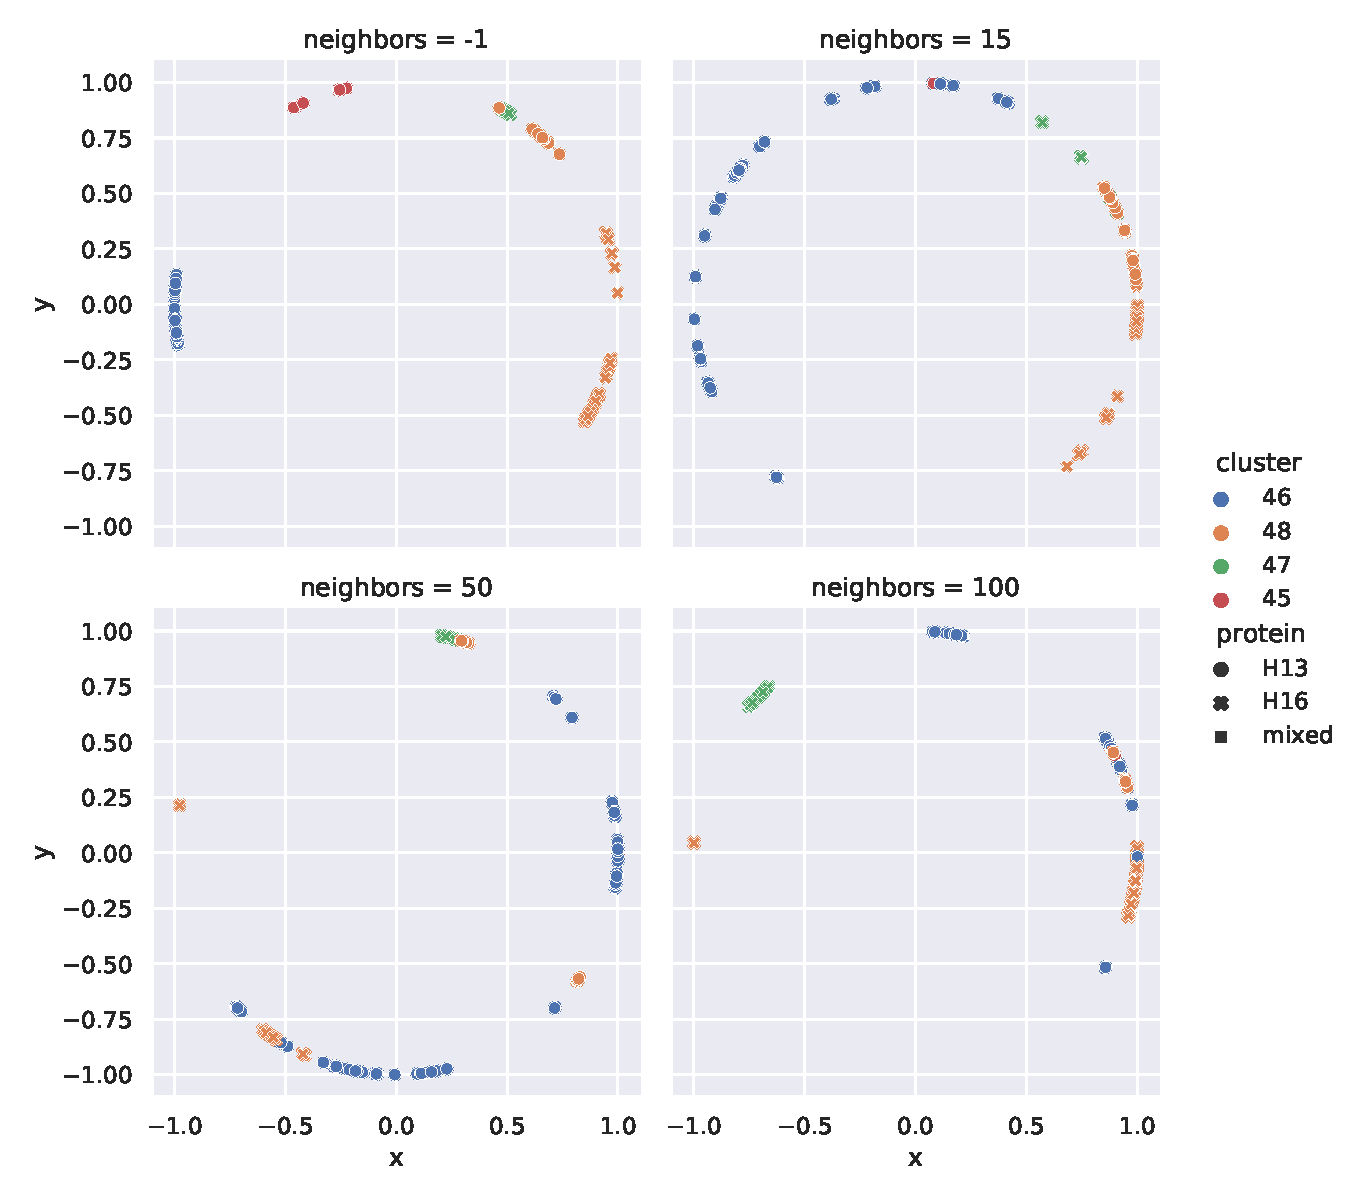
\includegraphics[width=\textwidth]{PCA/Difference_Segment_4_H_metric_cosine.pdf}
    \caption[H13/H16 Component Reduction Example (\Acrshort{PCA})]{\textbf{H13/H16 Component Reduction Example (\Acrshort{PCA}).} .}
    \label{fig:Reduction_Example_PCA}
\end{figure}

%wichtig erkläre warum dimension reuction mit neigbors 100 und dann feines clustering sinn macht -> HDBSCAN in methoden